% ===========================================================================
%  Does Economic Concept Selection Matter for Monetary Policy Shock Identification?
%  Three Tests on Aruoba & Drechsel (2024)
%  Compiled with: xelatex
% ===========================================================================
\documentclass[10pt,aspectratio=169]{beamer}
\usepackage{fontspec}
\usepackage{graphicx}
\usepackage{booktabs}
\usepackage{xcolor}
\usepackage{tikz}
\usetikzlibrary{positioning}
\usetheme{metropolis}
\setbeamercolor{frametitle}{bg=white,fg=black}
\setbeamercolor{title separator}{fg=blue!60!black}
\setbeamercolor{progress bar}{fg=blue!60!black}
\setbeamercolor{normal text}{fg=black}
\setbeamerfont{frametitle}{size=\Large,series=\bfseries}
\setbeamertemplate{navigation symbols}{}

\title{Does Economic Concept Selection Matter for Monetary Policy Shock Identification?}
\subtitle{Evidence from Aruoba \& Drechsel (2024)}
\date{May 2026}

\begin{document}

% ===== 1: TITLE =====
{
\setbeamertemplate{footline}{}
\begin{frame}[plain]
  \vspace{1.5cm}
  \begin{center}
    {\Huge\bfseries Does Economic Concept Selection\\[6pt] Matter for Monetary Policy Shock Identification?}\\[14pt]
    {\Large Evidence from Aruoba \& Drechsel (2024)}\\[16pt]
    {\normalsize Huang Zheng}\\[4pt]
    {\normalsize Monetary Policy \& Financial Markets}\\[4pt]
    {\normalsize May 2026}
  \end{center}
\end{frame}
}

% ======================================================================
% ACT 1: REPLICATION + METHOD
% ======================================================================

% ===== 2: AD(2024) METHOD =====
\begin{frame}{AD(2024) Scores Sentiment with a Dictionary}
  \vspace{2pt}
  \begin{center}
    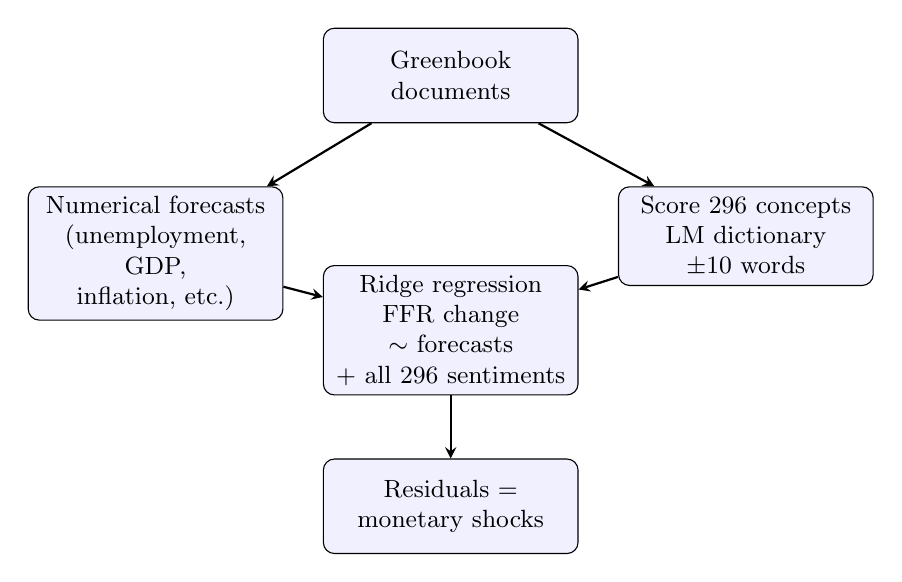
\begin{tikzpicture}[node distance=1.6cm, auto]
      \tikzstyle{block} = [rectangle, draw, fill=blue!6, text width=3.0cm, text centered, rounded corners, minimum height=1.2cm, font=\small]
      \tikzstyle{arrow} = [thick,->,>=stealth]
      \node[block] (A) {Greenbook\\documents};
      \node[block, below left=0.8cm and 0.5cm of A] (B1) {Numerical forecasts\\(unemployment, GDP,\\inflation, etc.)};
      \node[block, below right=0.8cm and 0.5cm of A] (B2) {Score 296 concepts\\LM dictionary $\pm$10 words};
      \node[block, below=1.8cm of A] (C) {Ridge regression\\FFR change $\sim$ forecasts\\$+$ all 296 sentiments};
      \node[block, below=0.8cm of C] (D) {Residuals =\\monetary shocks};
      \draw[arrow] (A) -- (B1);
      \draw[arrow] (A) -- (B2);
      \draw[arrow] (B1) -- (C);
      \draw[arrow] (B2) -- (C);
      \draw[arrow] (C) -- (D);
    \end{tikzpicture}
  \end{center}
  \vspace{6pt}
  \begin{block}{Headline result}
    \centering
    Full model (3,226 vars): \textbf{R$^2$ = 0.94}. \quad 94\% of FFR changes = systematic policy.
  \end{block}
\end{frame}

% ===== 3: REPLICATION OVERVIEW =====
\begin{frame}{First: We Replicated the Original Results}
  \vspace{4pt}
  \begin{columns}[T]
    \begin{column}{0.45\textwidth}
      \begin{block}{Table 2 — Forecast Error Predictability}
        \centering\small
        \begin{tabular}{lccc}
          \toprule
          Horizon & Our R$^2$ & Paper \\
          \midrule
          Current Q & 0.045 & 0.045 \\
          1Q ahead  & 0.149 & 0.149 \\
          \textbf{1Y ahead} & \textbf{0.248} & \textbf{0.248} \\
          2Y ahead  & 0.208 & 0.208 \\
          \bottomrule
        \end{tabular}
        \vspace{2pt}
        {\footnotesize PC1 of 296 sentiments $\to$ forecast errors.\\All horizons match exactly.}
      \end{block}
    \end{column}
    \begin{column}{0.55\textwidth}
      \begin{block}{Table 3 — First-Stage Fit}
        \centering\footnotesize
        \begin{tabular}{lccc}
          \toprule
          Specification & Vars & Our R$^2$ & Paper \\
          \midrule
          (4) Fc + sentiments & 429 & 0.64 & 0.65 \\
          (7) Full spec & 3,258 & 0.96 & 0.94 \\
          \bottomrule
        \end{tabular}
        \vspace{2pt}
        {\footnotesize Paper: R glmnet ($\alpha=0$). Ours: sklearn RidgeCV.\\$\sim$0.01 diff = CV lambda grid variation.}
      \end{block}
    \end{column}
  \end{columns}
  \vspace{6pt}
  \begin{center}
    \small\textbf{Both tables reproduced.} Data and pipeline verified.
  \end{center}
\end{frame}

% ===== 4: TABLE 3 FULL DATA =====
\begin{frame}{We Reproduce Table 3 Across All Specifications}
  \vspace{-2pt}
  \begin{center}
    \footnotesize
    \begin{tabular}{lccc}
      \toprule
      \textbf{Specification} & \textbf{Vars} & \textbf{Our R$^2$} & \textbf{Paper} \\
      \midrule
      (1) Romer-Romer OLS (basic forecasts)          & 17    & 0.46 & 0.50 \\
      (2) Ridge with extended forecasts              & 132   & 0.50 & 0.55 \\
      (3) + nonlinear forecasts                      & 298   & 0.51 & 0.51 \\
      (4) + all 296 sentiments (linear)              & 445   & 0.64 & 0.65 \\
      (5) + nonlinear sentiments                     & 890   & 0.74 & 0.75 \\
      (6) + 4 lags of sentiments (linear)            & 1,629 & 0.69 & 0.87 \\
      (7) \textbf{Full spec: + lags, nonlinear}      & \textbf{3,258} & \textbf{0.96} & \textbf{0.94} \\
      \bottomrule
    \end{tabular}
  \end{center}
  \vspace{4pt}
  \begin{block}{}
    \centering\small
    Ridge, 10-fold CV (R glmnet $\alpha=0$ vs.\ sklearn RidgeCV). All specs reproduced within CV margin.\\[2pt]
    Specs (4)--(7) include the 296 sentiment indicators --- these are what we test below.
  \end{block}
\end{frame}

% ======================================================================
% ACT 2: THE METHOD IS ROBUST — SENTIMENT ADDS VALUE EVERYWHERE
% ======================================================================

% ===== 5: SAMPLE SPLIT =====
\begin{frame}{Sentiment Adds Value Under Volcker, Greenspan, and Bernanke}
  \vspace{-6pt}
  \begin{center}
    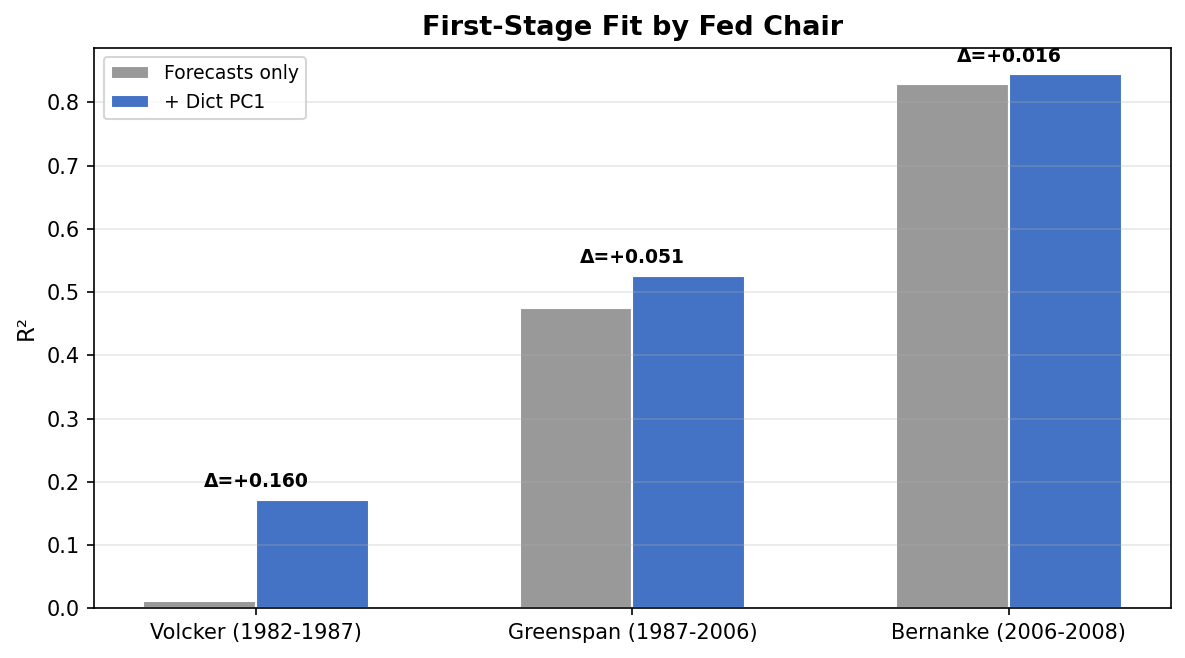
\includegraphics[width=0.68\textwidth]{figures/check1_sample_split.png}
  \end{center}
  \vspace{-10pt}
  \begin{block}{}
    \centering\scriptsize
    FFR change $\sim$ extended forecasts (gray) \quad vs.\quad FFR change $\sim$ extended forecasts + Dict PC1 (blue)
  \end{block}
  \vspace{0pt}
  \begin{columns}[T]
    \begin{column}{0.33\textwidth}
      \centering\scriptsize\textbf{Volcker (1982--87)}\\
      $n=39$. Discretionary. \quad $\Delta$R$^2$ = \textbf{+0.16}
    \end{column}
    \begin{column}{0.33\textwidth}
      \centering\scriptsize\textbf{Greenspan (1987--06)}\\
      $n=143$. Great Moderation. \quad $\Delta$R$^2$ = \textbf{+0.05}
    \end{column}
    \begin{column}{0.33\textwidth}
      \centering\scriptsize\textbf{Bernanke (2006--08)}\\
      $n=22$. Pre-crisis. \quad $\Delta$R$^2$ = \textbf{+0.02}
    \end{column}
  \end{columns}
\end{frame}

% ======================================================================
% ACT 3: BUT CONCEPT SELECTION IS SUBJECTIVE
% ======================================================================

% ===== 6: WHERE CONCEPTS COME FROM =====
\begin{frame}{The 296 Concepts Were Hand-Picked by the Authors}
  \begin{columns}[T]
    \begin{column}{0.52\textwidth}
      \vspace{4pt}
      \begin{block}{How the list was built}
        \begin{enumerate}
          \item Pull n-grams from 787 Greenbook PDFs
          \item Sort by document frequency
          \item \textbf{Authors manually pick} which ones are ``economic concepts''
          \item Final list: 296
        \end{enumerate}
      \end{block}
      \vspace{6pt}
      \begin{alertblock}{}
        \centering
        \textit{If someone else did step 3,\\would they pick the same 296?}
      \end{alertblock}
    \end{column}
    \begin{column}{0.48\textwidth}
      \begin{center}
        {\scriptsize A few of the 296 \ldots}\\[4pt]
        {\footnotesize
        \begin{tabular}{l}
          \texttt{advanced foreign economies}\\
          \texttt{business confidence}\\
          \texttt{consumer sentiment}\\
          \texttt{domestic final purchases}\\
          \texttt{economic expansion}\\
          \texttt{emerging market economies}\\
          \texttt{equity price}\\
          \texttt{foreign net purchases}\\
        \end{tabular}}
      \end{center}
    \end{column}
  \end{columns}
\end{frame}

% ===== 6: LLM DOES IT =====
\begin{frame}{We Replaced the Human Curator with an LLM}
  \vspace{2pt}
  \begin{block}{}
    \small Same 2,000 candidate n-grams from the same 787 texts.\\
    LLM reads each one: \textit{``economic concept or not? Which category?''}
  \end{block}
  \vspace{4pt}
  \begin{center}
    \large\textbf{The LLM picked \textcolor{blue!60!black}{595} concepts.}
    \quad\normalsize (The original authors picked 296.)
  \end{center}
  \vspace{4pt}
  \begin{columns}[T]
    \begin{column}{0.48\textwidth}
      \begin{block}{By category}
        \vspace{-4pt}\footnotesize
        \begin{tabular}{lr}
          Real activity & 204 \\
          Financial     & 150 \\
          Prices        & 99  \\
          International & 51  \\
          Labor         & 48  \\
          Fiscal/other  & 43  \\ \midrule
          \textbf{Total} & \textbf{595} \\
        \end{tabular}
      \end{block}
    \end{column}
    \begin{column}{0.52\textwidth}
      \begin{block}{}
        \footnotesize
        \begin{itemize}
          \item Nearly \textbf{twice as many}
          \item More coverage of financial, price, and international terms
          \item Did it agree with the human list on specifics?
        \end{itemize}
      \end{block}
    \end{column}
  \end{columns}
\end{frame}

% ===== 7: VENN =====
\begin{frame}{Human and LLM Agreed on Only 62.6\% of Concepts}
  \vspace{-6pt}
  \begin{center}
    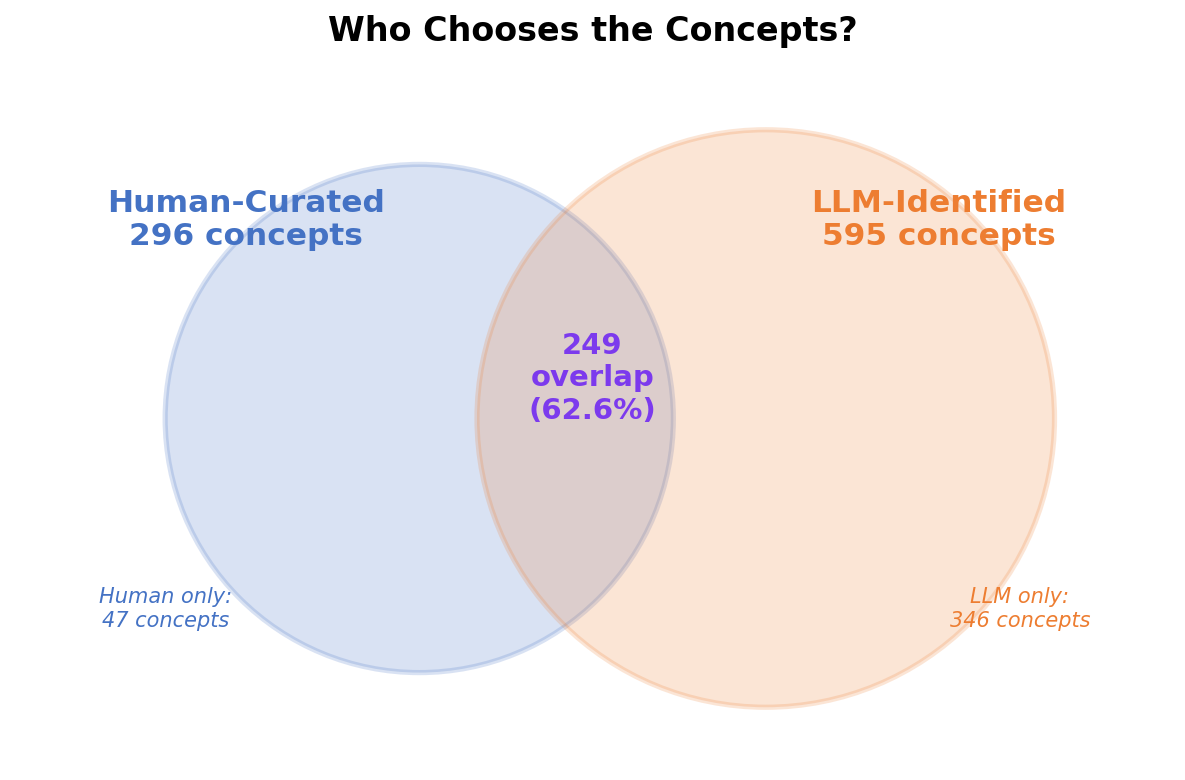
\includegraphics[width=0.52\textwidth]{figures/venn_human_vs_ai.png}
  \end{center}
  \vspace{-8pt}
  \begin{center}
    \footnotesize Human: 296 \hspace{16pt} LLM: 595 \hspace{16pt} Overlap: 249\\[4pt]
    \small Same texts, same 2,000 candidates. Different classifier. \textbf{37.4\% disagreement}.\\[2pt]
    {\scriptsize\color{gray} AD(2024): ``n-gram frequency analysis + manual screening.''\\
    The frequency step is mechanical. The screening is not.}
  \end{center}
\end{frame}

% ===== 8: SIDE-BY-SIDE =====
\begin{frame}{Humans Chose Specific Terms; the LLM Chose Broad Ones}
  \vspace{-4pt}
  \begin{columns}[T]
    \begin{column}{0.32\textwidth}
      \begin{block}{Only human picked}
        \centering\footnotesize\textit{specific, concrete}\\[2pt]
        \begin{tabular}{l}
          domestic final purchases\\
          district banks\\
          business confidence\\
          consumer sentiment\\
          drilling activity\\
          employment cost\\
        \end{tabular}
      \end{block}
    \end{column}
    \begin{column}{0.36\textwidth}
      \begin{block}{Both picked (249)}
        \centering\footnotesize\textit{agreed by both}\\[2pt]
        \begin{tabular}{l}
          inflation\\
          unemployment\\
          gdp growth\\
          housing starts\\
          exports\\
          credit\\
        \end{tabular}
      \end{block}
    \end{column}
    \begin{column}{0.32\textwidth}
      \begin{block}{Only LLM picked}
        \centering\footnotesize\textit{broad, general}\\[2pt]
        \begin{tabular}{l}
          prices\\
          markets\\
          labor\\
          federal reserve\\
          growth\\
          energy\\
        \end{tabular}
      \end{block}
    \end{column}
  \end{columns}
  \vspace{4pt}
  \begin{center}
    \small Human: specific. \quad LLM: broad. \quad \textbf{Different taste, not right vs.\ wrong.}
  \end{center}
  \vspace{2pt}
  \begin{block}{}
    {\scriptsize\color{gray} Prompt: \textit{``You are an economist. For each term, decide: is this an economic concept?''
    Yes/No + category. 50 terms per batch. Temperature = 0.1.}}
  \end{block}
\end{frame}

% ======================================================================
% ACT 4: THE ANXIETY + PLACEBO TEST
% ======================================================================

% ===== 9: ANXIETY =====
\begin{frame}{If Concept Selection Is Subjective, How Much Does It Matter?}
  \vspace{10pt}
  \begin{center}
    \Large Concept selection is fundamentally \textbf{subjective}.\\[14pt]
    Yet the headline --- \textbf{R$^2$ = 0.94} --- rests on\\[4pt]
    the exact list those particular authors settled on.\\[18pt]
    \Large\textbf{How much of the result is about the words chosen,}\\[4pt]
    \textbf{and how much is about the scoring method itself?}\\[18pt]
    \large An extreme test: \textbf{shuffle all concept labels. Re-run everything.}
  \end{center}
\end{frame}

% ===== 10: PLACEBO METHOD =====
\begin{frame}{We Shuffle All Concept Labels, Then Re-Run the Regression}
  \vspace{-4pt}
  \begin{center}
    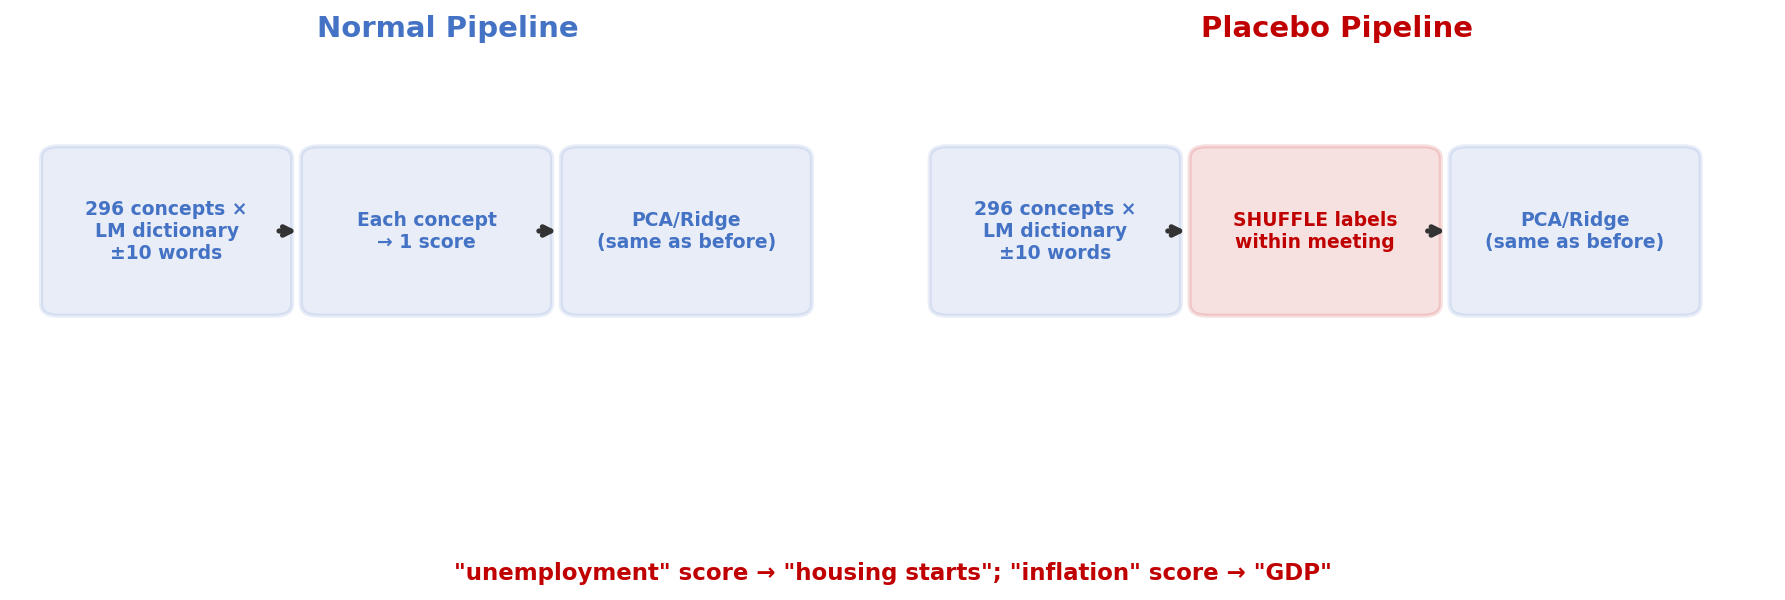
\includegraphics[width=0.82\textwidth]{figures/placebo_method.png}
  \end{center}
  \vspace{-4pt}
  \begin{block}{}
    \centering\small
    For each meeting, randomly permute the 296 scores across columns.\\
    ``Unemployment'' gets ``housing starts''' score. ``Inflation'' gets ``GDP'''s score.\\[2pt]
    Same scoring. Same regression. Same number of variables. \textbf{Only the labels change.}
  \end{block}
\end{frame}

% ===== 11: SHUFFLE DATA EXAMPLE =====
\begin{frame}{The Shuffle Scrambles Scores Within Each Meeting}
  \vspace{-2pt}
  \begin{columns}[T]
    \begin{column}{0.48\textwidth}
      \begin{block}{Before shuffle (correct labels)}
        \centering\footnotesize
        \begin{tabular}{lcccc}
          & \textbf{unemp.} & \textbf{inflat.} & \textbf{GDP} & \textbf{credit} \\
          \midrule
          Meeting 1 & $+0.3$ & $-0.1$ & $+0.5$ & $-0.2$ \\
          Meeting 2 & $-0.4$ & $+0.2$ & $-0.1$ & $+0.0$ \\
          Meeting 3 & $+0.1$ & $-0.3$ & $+0.4$ & $-0.1$ \\
        \end{tabular}
      \end{block}
    \end{column}
    \begin{column}{0.48\textwidth}
      \begin{block}{After shuffle (labels permuted)}
        \centering\footnotesize
        \begin{tabular}{lcccc}
          & \textbf{unemp.} & \textbf{inflat.} & \textbf{GDP} & \textbf{credit} \\
          \midrule
          Meeting 1 & $-0.1$ & $-0.2$ & $+0.3$ & $+0.5$ \\
          Meeting 2 & $+0.0$ & $+0.2$ & $-0.1$ & $-0.4$ \\
          Meeting 3 & $-0.3$ & $-0.1$ & $+0.1$ & $+0.4$ \\
        \end{tabular}
      \end{block}
    \end{column}
  \end{columns}
  \vspace{4pt}
  \begin{center}
    \small Within each row, the \textbf{same 4 numbers} --- just in different columns.\\[2pt]
  \end{center}
  \begin{block}{}
    \centering\footnotesize\ttfamily
    for i in range(n): ~~X\_shuffled[i, :] = rng.permutation(X\_sent[i, :])
  \end{block}
\end{frame}

% ===== 12: TEST 1 — MID SPEC =====
\begin{frame}{With 429 Variables, Shuffling Labels Changes Nothing}
  \vspace{4pt}
  \begin{block}{Specification}
    \centering\small
    132 extended forecasts $+$ 296 sentiment indicators $\to$ Ridge, 10-fold CV. \quad 429 vars.
  \end{block}
  \vspace{8pt}
  \begin{center}
    \begin{tabular}{c}
      {\large Correct labels}\\[2pt]
      {\Huge R$^2$ = 0.64}\\[12pt]
      {\large Shuffled labels \hspace{6pt} (mean of 100 permutations)}\\[2pt]
      {\Huge R$^2$ = 0.65}\\[12pt]
      {\Large\textcolor{blue!60!black}{\textbf{No drop.}}}
    \end{tabular}
  \end{center}
\end{frame}

% ===== 13: WHY =====
\begin{frame}{All 296 Scores Point the Same Way Within a Meeting}
  \vspace{-8pt}
  \begin{center}
    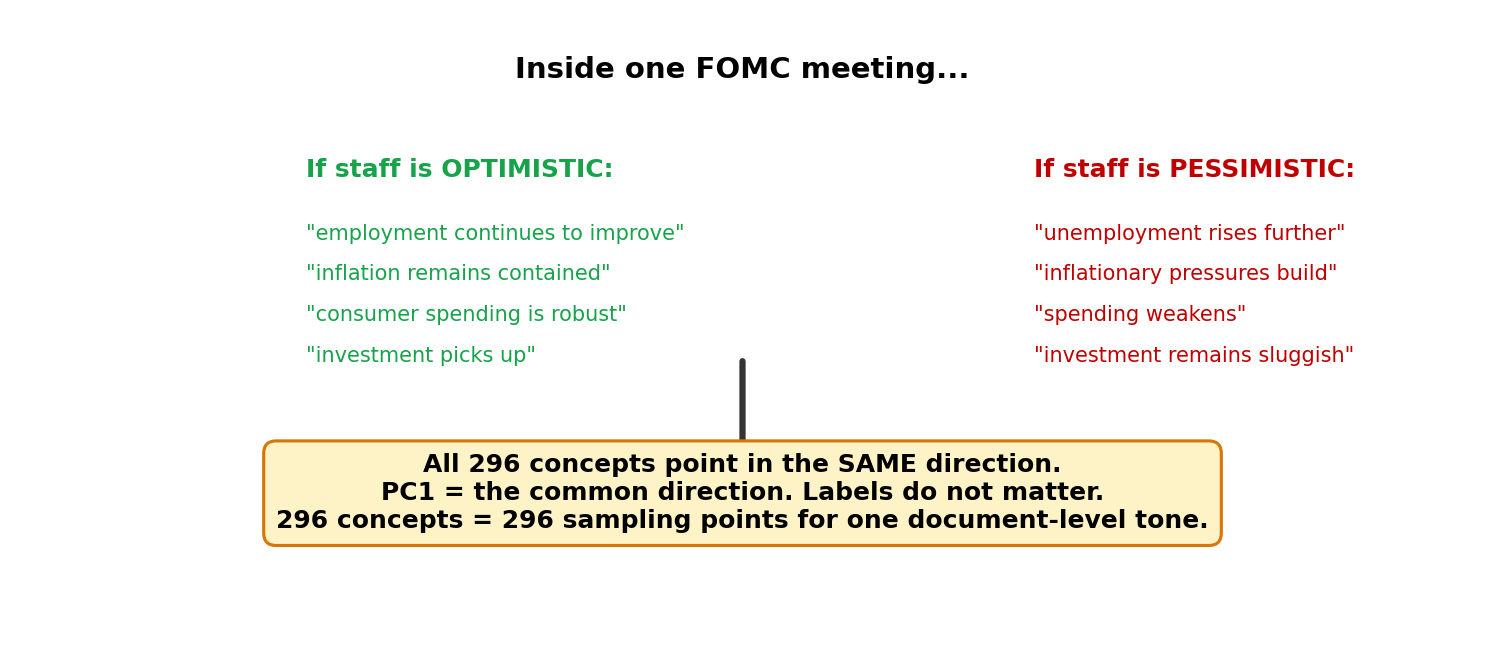
\includegraphics[width=0.78\textwidth]{figures/why_pc1_works.png}
  \end{center}
\end{frame}

% ===== 14: TEST 2 — FULL SPEC =====
\begin{frame}{With 3,224 Variables, Shuffling Drops R² by Only 0.03}
  \vspace{2pt}
  \begin{block}{Specification}
    \centering\footnotesize\ttfamily
    X = np.column\_stack([X\_forecasts, X\_forecasts**2,\\
    \hspace{8pt} X\_sentiments, X\_sentiments**2,\\
    \hspace{8pt} X\_sentiments\_lag1, ..., X\_sentiments\_lag4,\\
    \hspace{8pt} X\_sentiments\_lag1**2, ..., X\_sentiments\_lag4**2])\\
    ridge = RidgeCV(cv=10).fit(X, y)
  \end{block}
  \vspace{2pt}
  \begin{center}
    \begin{tabular}{c}
      {\large Correct labels: \textbf{R$^2$ = 0.96}}\\[4pt]
      {\large Shuffled labels (mean of 50): \textbf{R$^2$ = 0.93}}\\[4pt]
      {\Large\textcolor{blue!60!black}{\textbf{Dropped by 0.03.}}}
    \end{tabular}
  \end{center}
\end{frame}

% ======================================================================
% ACT 5: SUMMARY + DEEP DIVE
% ======================================================================

% ===== 15: SHUFFLE COMPARISON CHART =====
\begin{frame}{Shuffling Labels: The Full Picture}
  \vspace{-4pt}
  \begin{center}
    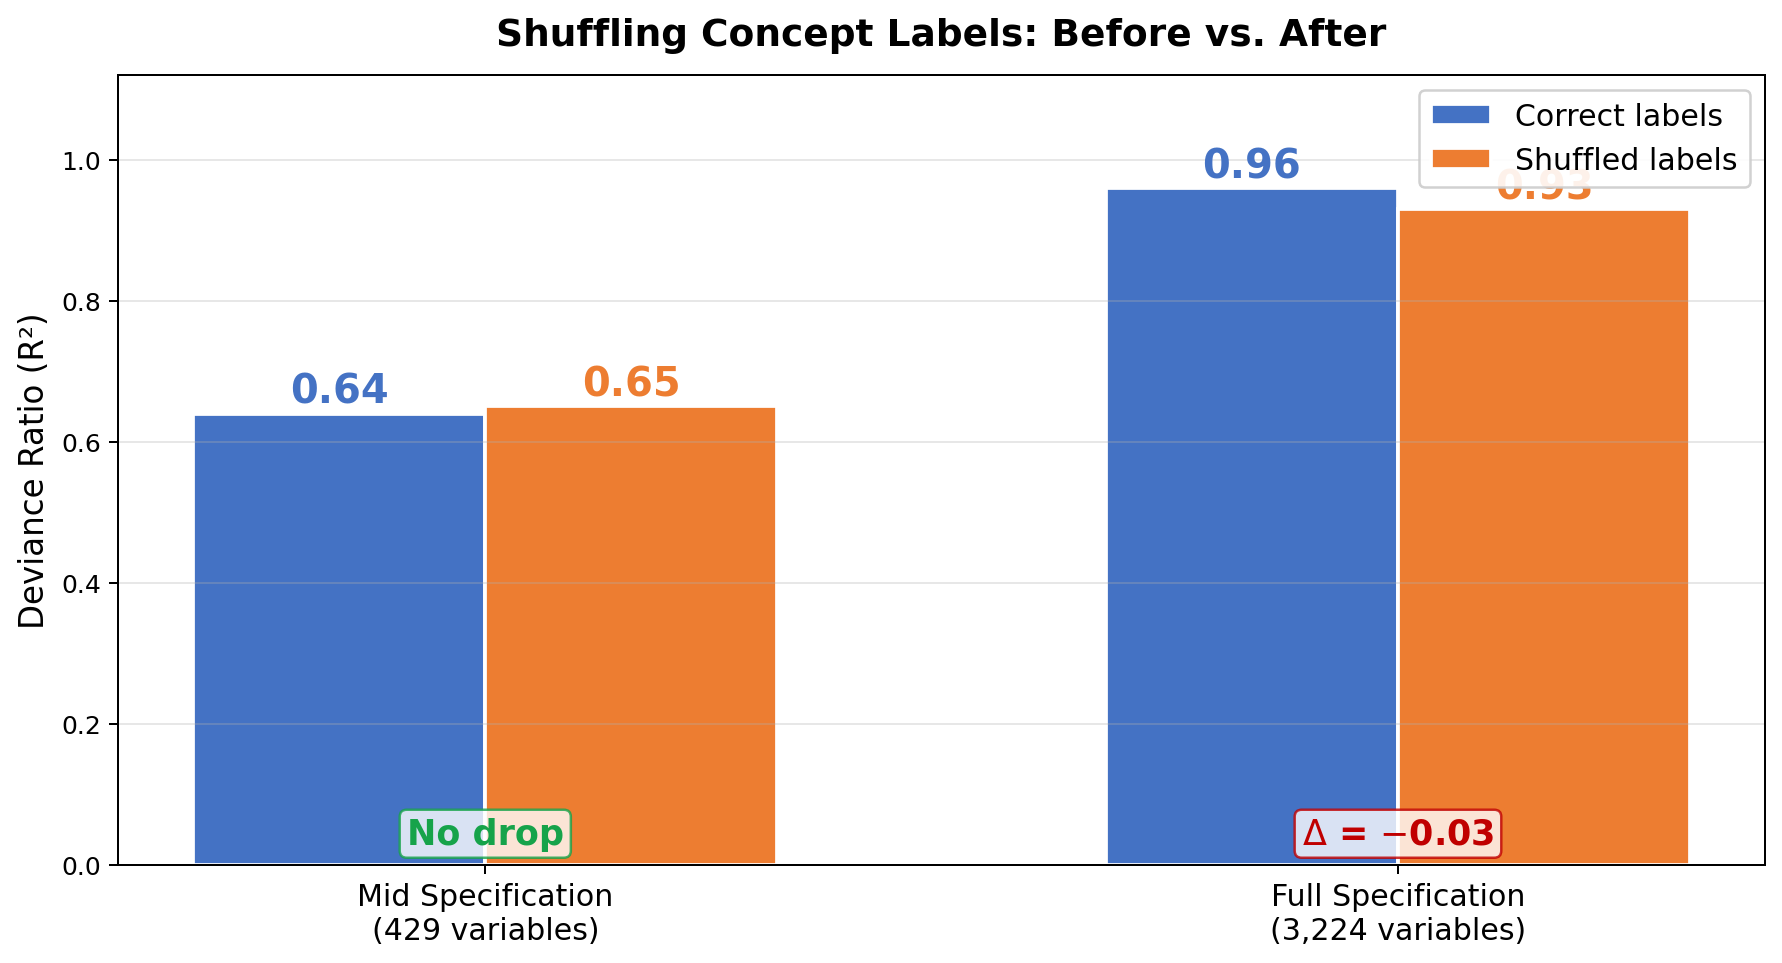
\includegraphics[width=0.78\textwidth]{figures/shuffle_comparison.png}
  \end{center}
  \vspace{-4pt}
  \begin{center}
    \small Mid spec: no effect. \quad Full spec: only 0.03 lost.\\
    \textbf{The concept labels themselves contribute almost nothing to the fit.}
  \end{center}
\end{frame}

% ===== 16: WATERFALL =====
\begin{frame}{The Scoring Method Contributes 10$\times$ More Than Label Identity}
  \vspace{-6pt}
  \begin{center}
    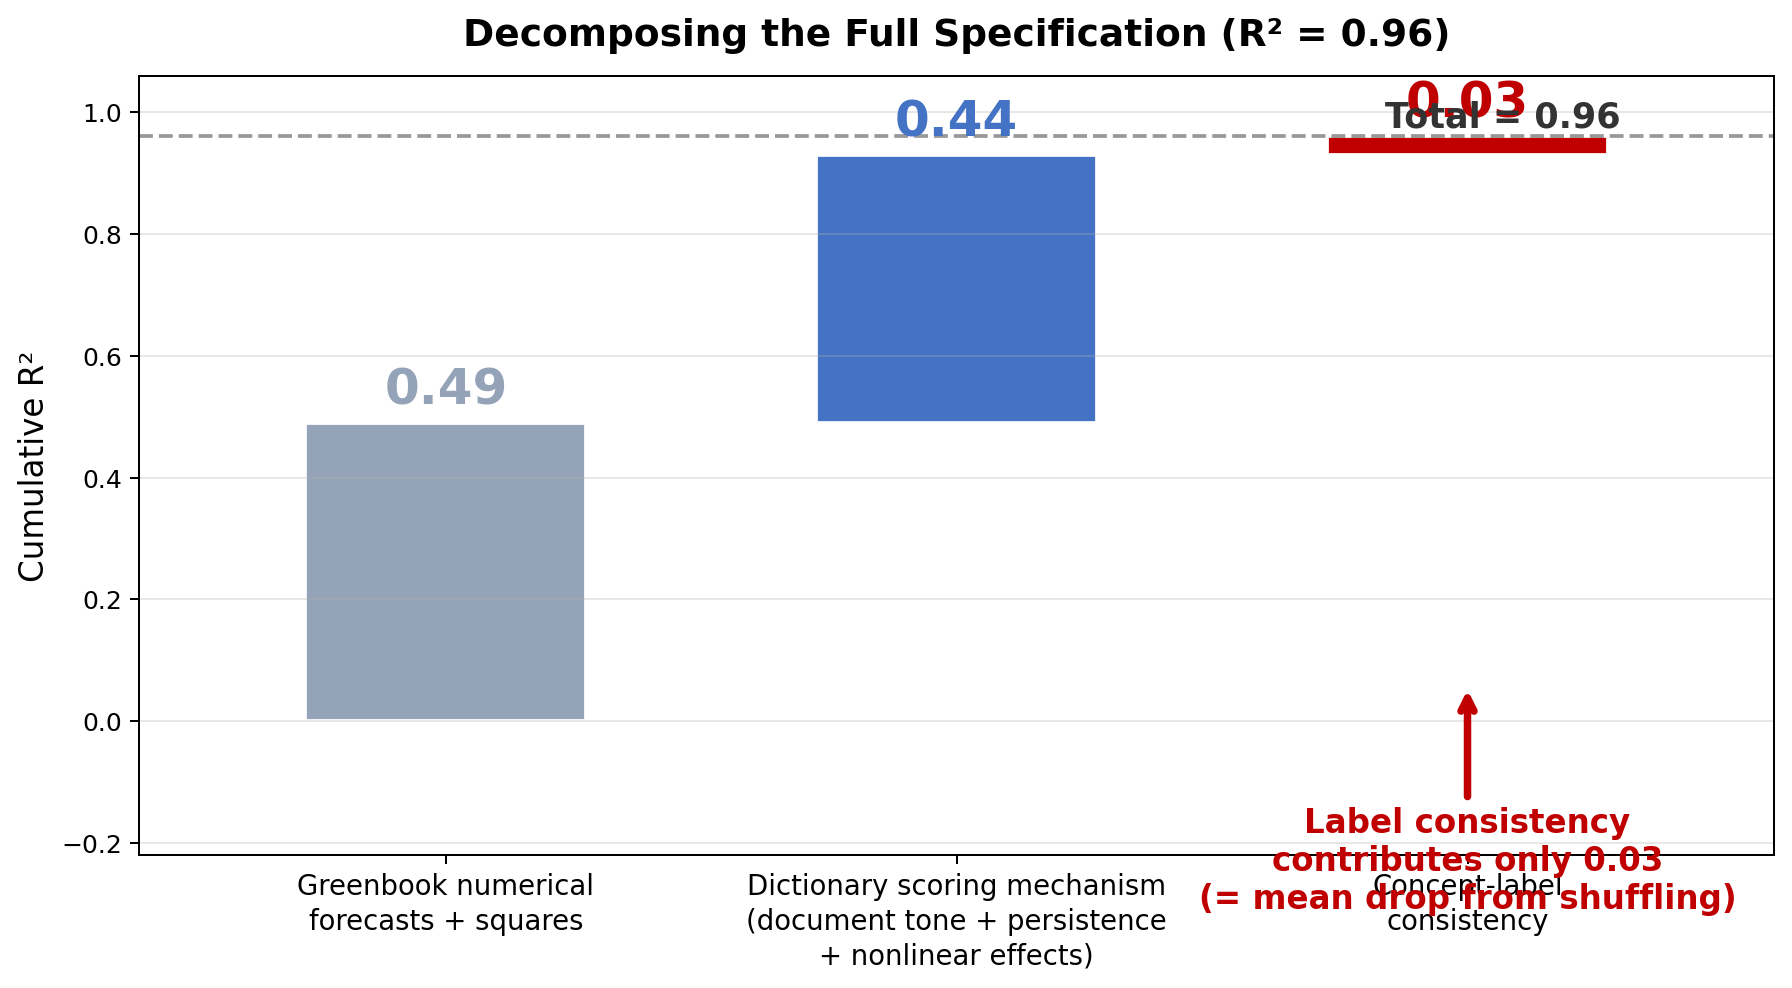
\includegraphics[width=0.92\textwidth]{figures/waterfall_decomposition.png}
  \end{center}
  \vspace{-8pt}
  \begin{center}
    \small Of the 0.96, only \textcolor{red!60!black}{0.04} depends on which word is which.
  \end{center}
\end{frame}

% ===== 17: WHY PLACEBO PASSED =====
\begin{frame}{The Original 296 Concepts Are Mostly Pro-Cyclical}
  \vspace{-4pt}
  \begin{center}
    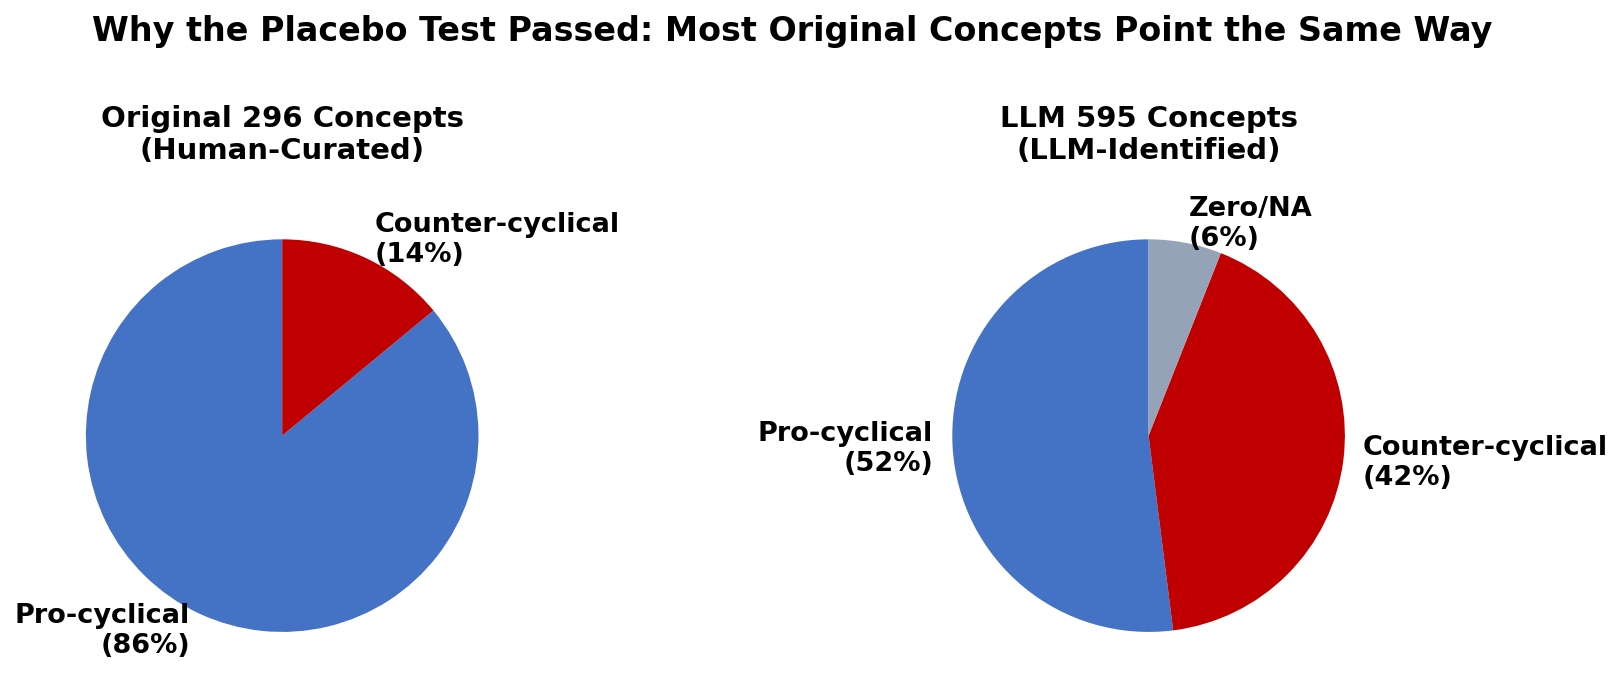
\includegraphics[width=0.82\textwidth]{figures/cyclicality_comparison.png}
  \end{center}
  \vspace{-6pt}
  \begin{center}
    \small 86\% of the original 296 move with the cycle. Only 14\% go the other way.\\
    \small The LLM's 595 are much more balanced (52\% vs.\ 42\%).\\[2pt]
    \textbf{The placebo test passed partly because the original list is already one-sided.}
  \end{center}
\end{frame}

% ===== 18: PRO-CYCLICAL EXPLAINER =====
\begin{frame}{What Does ``Pro-Cyclical'' Mean --- and Why Does It Matter?}
  \vspace{2pt}
  \begin{block}{Definition}
    \centering\small
    A concept is \textbf{pro-cyclical} if its sentiment score is positively correlated with PC1 (the common factor).\\
    When the economy is good, its score is positive. When bad, its score is negative. \textbf{It moves with the cycle.}
  \end{block}
  \vspace{4pt}
  \begin{columns}[T]
    \begin{column}{0.48\textwidth}
      \begin{block}{Example: pro-cyclical concepts}
        \centering\footnotesize
        \begin{tabular}{lr}
          \toprule
          Concept & Corr.\ with PC1 \\
          \midrule
          business activity   & $+$0.73 \\
          firms               & $+$0.72 \\
          manufacturing       & $+$0.71 \\
          employment          & $+$0.69 \\
          construction        & $+$0.68 \\
          \bottomrule
        \end{tabular}
        \vspace{2pt}
        Economy improves $\to$ positive language around these concepts $\to$ positive score.
      \end{block}
    \end{column}
    \begin{column}{0.48\textwidth}
      \begin{block}{Example: counter-cyclical concepts}
        \centering\footnotesize
        \begin{tabular}{lr}
          \toprule
          Concept & Corr.\ with PC1 \\
          \midrule
          output gap          & $-$0.33 \\
          potential output    & $-$0.32 \\
          uncertainty         & $-$0.25 \\
          federal debt        & $-$0.17 \\
          fiscal policy       & $-$0.15 \\
          \bottomrule
        \end{tabular}
        \vspace{2pt}
        Economy improves $\to$ cautious or negative language around these concepts.
      \end{block}
    \end{column}
  \end{columns}
  \vspace{4pt}
  \begin{block}{How we determine this}
    \centering\small
    For each concept, correlate its 204-meeting sentiment time series with PC1.\\
    \textbf{Positive correlation = pro-cyclical. Negative correlation = counter-cyclical.}
  \end{block}
  \vspace{2pt}
  \begin{alertblock}{Why this matters}
    \small
    The original 296 concepts are \textbf{86\% pro-cyclical}. Most point the same way in any given meeting.\\
    This is why shuffling labels barely matters --- the common signal dominates regardless of labels.\\
    A \textbf{more balanced} list (like the LLM's 52\%/42\%) would leave more room for labels to matter.\\[2pt]
    \textbf{Concept selection matters --- not which specific words, but the overall composition of the list.}
  \end{alertblock}
\end{frame}

% ======================================================================
% ACT 6: CONCLUSION
% ======================================================================

% ===== 20: CONCLUSION =====
\begin{frame}{Concept Selection Matters --- At the Level of List Composition}
  \vspace{6pt}
  \begin{block}{The method is robust across regimes}
    \centering\small
    Sentiment adds incremental R$^2$ under Volcker (+0.16), Greenspan (+0.05), and Bernanke (+0.02).\\
    The AD(2024) pipeline works. The question is \textbf{why}, and \textbf{where its limits are}.
  \end{block}
  \vspace{6pt}
  \begin{block}{The concept list is subjective --- but that barely matters for the result}
    \centering\small
    Human vs.\ LLM curation: only 62.6\% agreement. Yet shuffling all 296 labels drops R$^2$ by only 0.03.
  \end{block}
  \vspace{6pt}
  \begin{block}{Why? Because 86\% of the original concepts are pro-cyclical}
    \centering\small
    Most point the same way within any meeting. The common signal dominates regardless of labels.\\
    With a \textbf{more balanced} list (like the LLM's 52/42 split), shuffling could matter more.
  \end{block}
  \vspace{6pt}
  \begin{center}
    \large\textbf{Concept selection matters --- not which specific words, but how the list is composed.}
  \end{center}
\end{frame}

% ===== 21: THANK YOU =====
{
\setbeamertemplate{footline}{}
\begin{frame}[plain]
  \vspace{3cm}
  \begin{center}
    {\Huge Thank You}
  \end{center}
\end{frame}
}

\end{document}
